\input{../Common/commands}

\begin{document}

% has to be after begin doc
\setlength\parskip{1ex}

\graphicspath{ {../Common/images/} }
\input{../Common/map}
\graphicspath{ {images/} }

% ----------------------------------------------------------------
% PAGE TITLE
% ----------------------------------------------------------------
%{\reversemarginpar\marginnote{\bothhead}[-5cm]}
\pgclryellow
\title{\headerpres{Data Analysis: \\ Relationships Between Data}}
\author{\vspace{3cm} Institute of Technology Tallaght}
\date{Department of Computing}
\maketitle
\newpage

%===================================================================
% GENERAL
%===================================================================
\headerch{Relationships}
\begin{itemize}
\item Different relationships between data are of interest in data analysis:
  \begin{itemize}
  \item Relationships between \textbf{numerical data variables} (on the interval or ratio scale)
  \item Relationships between \textbf{data variables  on the nominal and ordinal scales}
  \item Relationships between \textbf{data set statistics}, such as the mean or  the standard deviation, for different variables
  \end{itemize}
\item Relationships can be examined using \textbf{visualisation} or expressed through mathematically calculated \textbf{measures}
\item NOTE: The existence of a relationship between two variables \emph{does not} imply that there is any causation involved.
\end{itemize}
\newpage

%===================================================================  
% VISUALISATION
%===================================================================
\headerch{Relationship visualisation}

Relationships can be discovered by examining suitable visual representations of data
\begin{itemize}
\item \textbf{Scatterplots}

  \oneex
  \begin{tabular}{m{0.25\textwidth}m{0.25\textwidth}m{0.25\textwidth}}
  {\small \emph{Positive relationship}} & {\small \emph{Negative relationship}} &{\small \emph{No relationship}} \\
  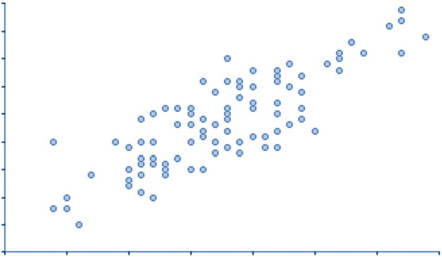
\includegraphics[width=0.25\textwidth]{pos_rel_vis.png} &
  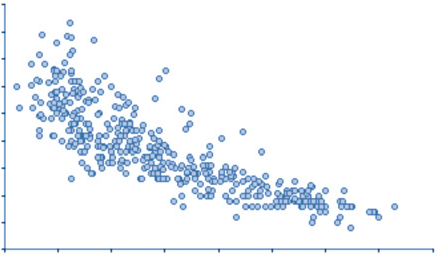
\includegraphics[width=0.25\textwidth]{neg_rel_vis.png} &
  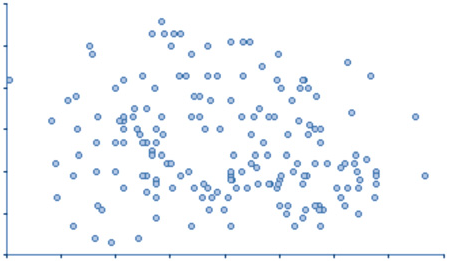
\includegraphics[width=0.25\textwidth]{no_rel_vis.png} \\ [-1.5ex] 
    {\fontsize{10}{0}\selectfont \textbf{Source: [MSD]}} &
    {\fontsize{10}{0}\selectfont \textbf{Source: [MSD]}} &
    {\fontsize{10}{0}\selectfont \textbf{Source: [MSD]}} \\    
  \end{tabular}
  \newpage

\item \textbf{Summary tables and graphs} \\
  To show data in a summary table or graph, the data is grouped based on the values of a discrete variable or ranges of a continuous variable. The table or graph summarises properties of a numeric variable for each group.
  \begin{itemize}
  \item Summary table
    \begin{itemize}
    \item Each data subset is shown in a row of the table
    \item One of the columns usually contains observation counts for the subsets
    \item The remaining columns represent properties, such as mean or standard deviation, of a numeric variable 
    \end{itemize}
    \twoex
    \begin{tabular}{l}
    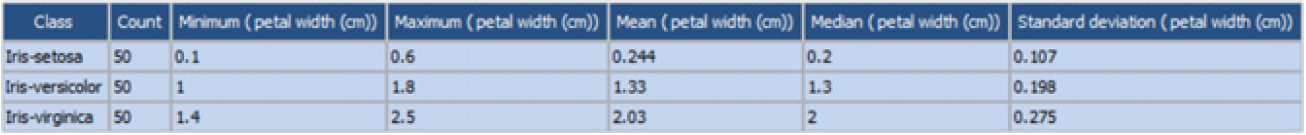
\includegraphics[width=0.9\textwidth]{sum_tab_vis.png}\\ [-1.5ex]
    {\fontsize{10}{0}\selectfont \textbf{Source: [MSD]}} \\
    \parbox{0.9\textwidth}{\halfex \tiny \emph{The data in the table above is grouped by type of iris. The columns represent properties of the variable ''petal width''. The table is immediately informative, showing the  marked difference between the petal width of the three classes of iris.}} \\
    \end{tabular}
    \newpage
  \item Summary graph
    \begin{itemize}
    \item A graphical representation of the data shown in a summary table 
    \item The grouping variable from the summary table is on the x-axis
      \item The y-axis represents a property of the other variable
      \end{itemize}
     \twoex
    \begin{tabular}{ll}
      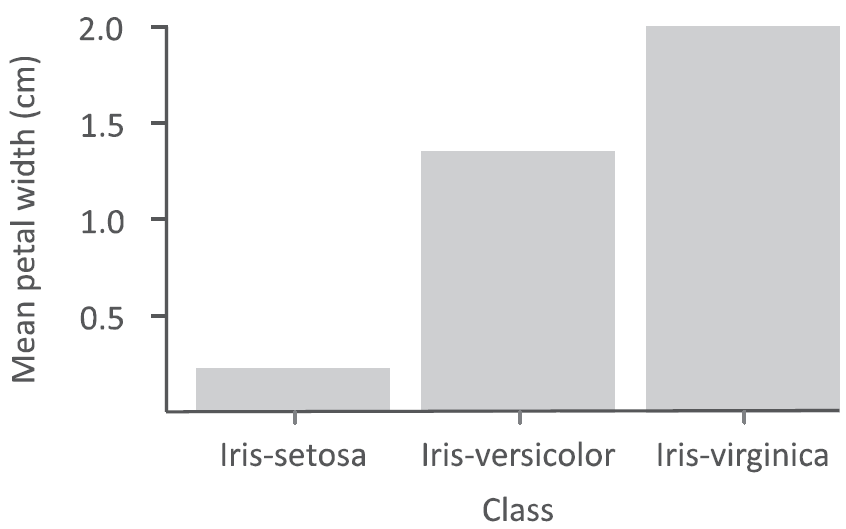
\includegraphics[width=0.4\textwidth]{sum_bch_vis.png}&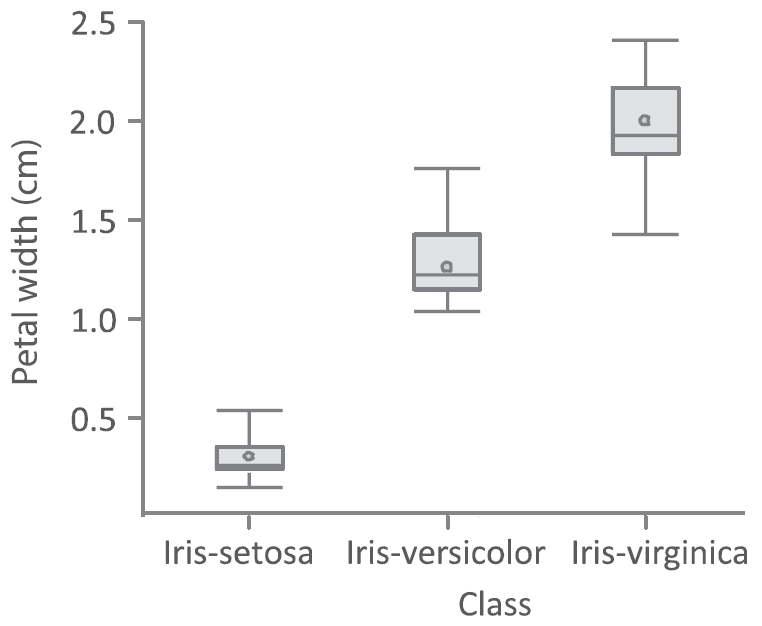
\includegraphics[width=0.35\textwidth]{sum_box_vis.png} \\ [-1.5ex]
       {\fontsize{10}{0}\selectfont \textbf{Source: [MSD]}}&{\fontsize{10}{0}\selectfont \textbf{Source: [MSD]}} \\ [1ex]
    \multicolumn{2}{l}{\parbox{0.8\textwidth}{\tiny \emph{These two summary diagrams are of the mean petal width and of petal width box and whisker visualisations for the different iris classes. Comparing the classes is even easier than with the summary table.}}}
    \end{tabular}
  \end{itemize}
  \newpage

\item \textbf{Contingency table}
  \begin{itemize}
  \item Provides insight into the relationship between two categorical variables (or non-categorical variables converted to categorical). 
  \item Contains observation counts for each possible pair of values for the two variables
  \item Also called \emph{cross-classification} table
  \end{itemize}
  \twoex
  \begin{tabular}{ll}
  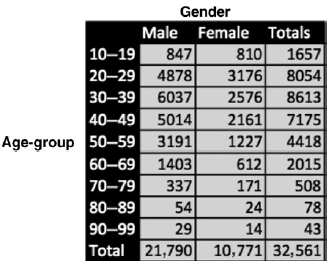
\includegraphics[width=0.4\textwidth]{cont_tab_vis.png}&
  \parbox[b][0.32\textwidth][t]{0.2\textwidth}{\tiny \emph{An example of a contingency table, showing counts for pairs of values for variables Gender and Age-group}} \\ [-1.5ex]
    {\fontsize{10}{0}\selectfont \textbf{Source: [MSD]}} & \\
  \end{tabular}
\end{itemize}
\newpage
%===================================================================
% MEASURES - STATISTICS
%===================================================================
\headerch{Measuring relatedness (statistics)}

A number of different measures are used for quantifying the degree of relatedness between variables. 
\begin{itemize}
  
% ----------------------------------------------------------------
% PEARSON COEFFICIENT
% ----------------------------------------------------------------
\item \textbf{Pearson's product-moment correlation coefficient}
  \begin{itemize}
  \item Most common correlation coefficient, often referred to simply as 'correlation coefficient'
  \item Defined by Karl Pearson (1857-1936), English mathematician and statistician 
  \item Measures linear correlation between two numeric variables (on interval or ratio scale)
  \item A number between -1.0 and 1.0, inclusive, expressing relatedness on a scale from \emph{perfect negative correlation} (-1.0) to \emph{perfect positive correlation} (1.0). A value of 0 means \emph{no correlation}.
    \newpage
    
  \item The formula for calculating the correlation coefficient is:
    $$ r = \dfrac{\displaystyle\sum_{i=1}^n (x_i - \mean{x})(y_i - \mean{y})}{(n-1)s_xs_y} $$    
    where $x$ and $y$ are variables, $x_i$ are the individual values of $x$, $y_i$ are the individual values of $y$, $\mean{x}$ is the mean of the $x$ variable, $\mean{y}$ is the mean of the $y$ variable, $s_x$ and $s_y$ are the standard deviations of variables $x$ and $y$, respectively, and $n$ is the number of observations.  
  \item Examples of two scatterplots with different values of correlation coefficient:
    
    \oneex
    $r=0.83$ \hspace{12em}  $r=0.59$ \\
    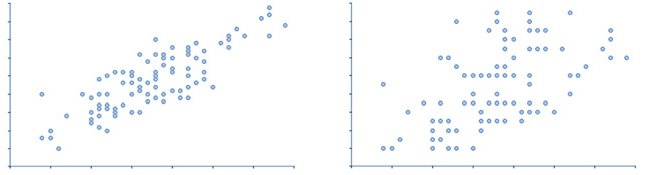
\includegraphics[width=0.8\textwidth]{correlation_examples.jpg}\\ [-1.5ex] 
    {\fontsize{10}{0}\selectfont \textbf{Source: [MSD]}}
    \newpage
  \item Testing the significance of Pearson's product-moment correlation coefficient
    \begin{itemize}
    \item For a pair of perfectly independent variables, the coefficient that is calculated on a pair of samples has a distribution with mean equal to 0 (see  \underline{\href{https://www.researchgate.net/figure/Distribution-of-Pearson-correlation-coefficient-of-stationary-series-with-autocorrelation_fig1_262056371}{here}}). 
    \item The smaller the sample size, the greater the correlation value needs to be in order to be considered significant (\underline{\href{https://en.wikipedia.org/wiki/Pearson_correlation_coefficient\#/media/File:Critical_correlation_vs._sample_size.svg}{Wikipedia picture illustrating this}}.)
    \item The critical values are always given in a table:

      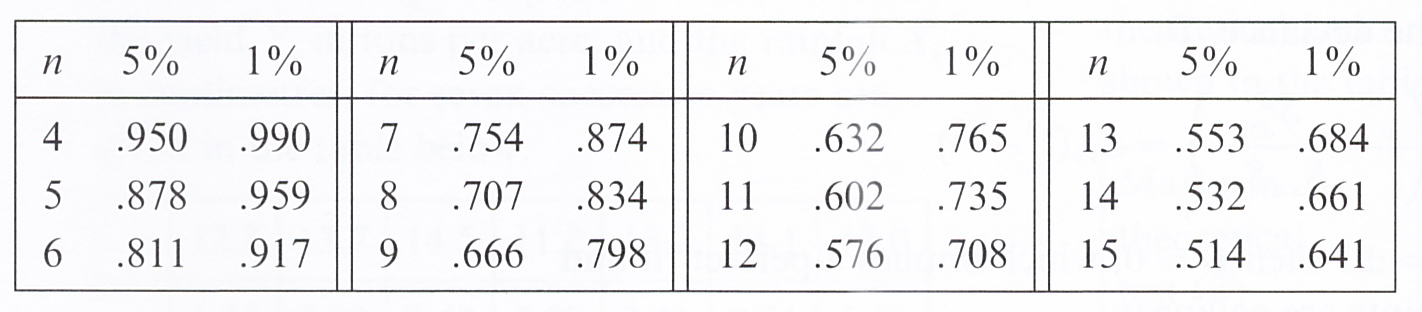
\includegraphics[width=0.8\textwidth]{2_1_1_r_significance_table.png}\\ [-1.5ex] 
      {\fontsize{10}{0}\selectfont \textbf{Source: [US]}}

     A larger table can be found \underline{\href{http://www.real-statistics.com/statistics-tables/pearsons-correlation-table/}{here}}. The degrees of freedom value is calculated as $df = N - 2$.
      
      
    \end{itemize}
  \end{itemize}
  \newpage


  
% ----------------------------------------------------------------
% KENDALL TAU
% ----------------------------------------------------------------
\item \textbf{Kendall Tau}
  \begin{itemize}
  \item Measures association betwen a pair of numeric variables (on the interval or ratio scale)
  \item Defined by English statistician Maurice Kendall (1907-1983)
  \item Also called \emph{Kendall rank correlation coefficient}
  \item Calculated using value \emph{ranks} rather than values, as follows:
    \begin{enumerate}
    \item Let's say that the variables are $X$ and $Y$, with values $x_1, x_2, ... x_n$ and  $y_1, y_2, ... y_n$, respectively, and pairs ${(x_1,y_1), (x_2, y_2), ... (x_n, y_n)}$ corresponding to observations. 
    \item Each value is given a \emph{rank} within the context of its variable, based on numeric value (the highest value receives rank 1 etc.). This means that the values for $X$ will have unique rank values between $1$ and $n$, as will the values for $Y$.  
    \item The pairs are tested with other pairs for \emph{concordance} vs. \emph{discordance}. The following table shows tested conditions and corresponding rank relationship designations.
\newpage
      {\tiny \setlength\extrarowheight{0.5em}
      \begin{tabular}{ll}
      \hline
      \textbf{Fulfilled condition} & \textbf{Concordance value for} \textbf{$(x_i, y_i)$ and $(x_j, y_j)$} \\
      \hline
      $r(x_i)-r(x_j) > 0$ AND $r(y_i)-r(y_j) > 0$ & concordant \\
      $r(x_i)-r(x_j) < 0$ AND $r(y_i)-r(y_j) < 0$ & concordant \\
      $r(x_i)-r(x_j) > 0$ AND $r(y_i)-r(y_j) < 0$ & discordant \\
      $r(x_i)-r(x_j) < 0$ AND $r(y_i)-r(y_j) > 0$ & discordant \\
      $r(x_i)-r(x_j) = 0$ & x-tied \\
      $r(y_i)-r(y_j) = 0$ & y-tied \\
      \hline
      \multicolumn{2}{l}{\textbf{NOTE:} $r(x_i)$ denotes the rank of value $x_i$ in the context of variable X etc.}\\
      \end{tabular}}
    \oneex
    \item The counts of concordant, discordant, x-tied and y-tied pairs ($n_c$, $n_d$, $t_x$ and $t_y$, respectively) are determined (note that a pair can be both x-tied and y-tied at the same time i.e. counted both in $t_x$ and in $t_y$). The counts are used in the calculation of the Tau value.
    \item There are two Tau calculations, $\tau_A$ and $\tau_B$, each resulting in values between $-1.0$ and 1.0. The former is simpler and is used when there are no ties. The Tau forumalae are:
    $$ \tau_A = \dfrac{n_c - n_d}{n(n-1)/2}$$
    $$ \tau_B = \dfrac{n_c - n_d}{\sqrt{(n_c+n_d+t_x)(n_c+n_d+t_y)}}$$
  \end{enumerate}

\item The significance of Kendall's Tau also depends on the sample size. We test it by looking it up in the table of Kendall Tau critical values:

      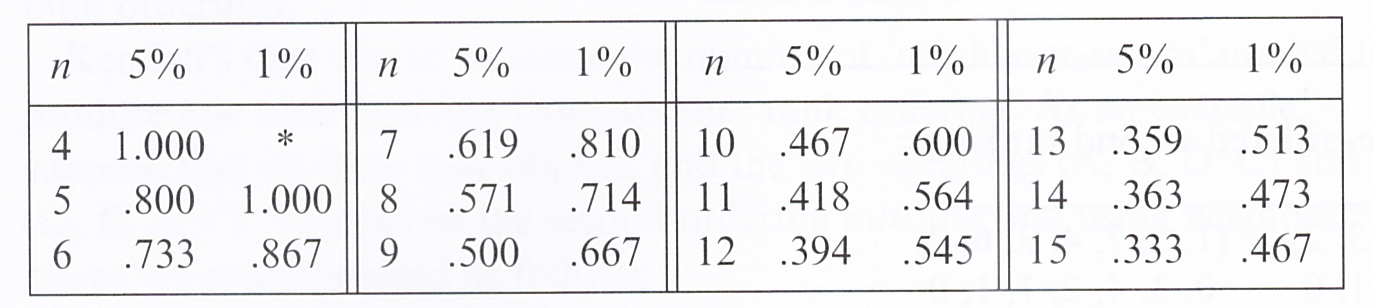
\includegraphics[width=0.8\textwidth]{2_1_1_tau_significance_table.png}\\ [-1.5ex] 
      {\fontsize{10}{0}\selectfont \textbf{Source: [US]}}
  \end{itemize}
  \newpage

% ----------------------------------------------------------------
% T-TESTS
% ----------------------------------------------------------------
\item \textbf{t-Tests for comparing two groups}
  \begin{itemize}
  \item Test the means of two groups of observations for whether the difference between their means is statistically significant (not likely to be due to expected variation in values)
  \item Take the form of hypothesis tests
  \item Is typically applied in cases where the number of instances is small (less than 30)
  \item The statistic used in a t-test is called a T value and is the difference between the two means, normalised to the standard error of the difference distribution
  \item The T value follows a t-distribution with a number of degrees of freedom that depends on the properties of the two variables 
  \item The formula for this value, in the case that the two groups are independently normally distributed and have similar variances, is: \\
    $$ T = \dfrac{\mean{x_1} - \mean{x_2}}{s_p\sqrt{\dfrac{1}{n_1}+\dfrac{1}{n_2}}} $$
    where $\mean{x_1}$ and $\mean{x_2}$ are the group means, $n_1$ and $n_2$ are group observation count and $s_p$ is an estimate of the standard deviation, calculated as follows: \\
    $$ s_p=\sqrt{\dfrac{(n_1-1)s_1^2+(n_2-1)s_2^2}{n_1+n_2-2}} $$
    where $s_1^2$ and $s_2^2$ are group variances. \\
    In this case the number of degrees of freedom is $df = n_1+n_2-2$.
  \item In the case that the group variances are not similar, a different, more complicated formula is used. 

  \item Testing the significance of a t statistic

    \begin{itemize}
      \item If the calculated value of T falls within a certain range in the middle of the relevant t-distribution (usually a range that includes 95\% of the distribution's values), it is taken that the difference between the two group means is not statistically significant i.e. that the means of the populations they represent are highly likely to be the same.

    \item t-statistic distribution graphs:

      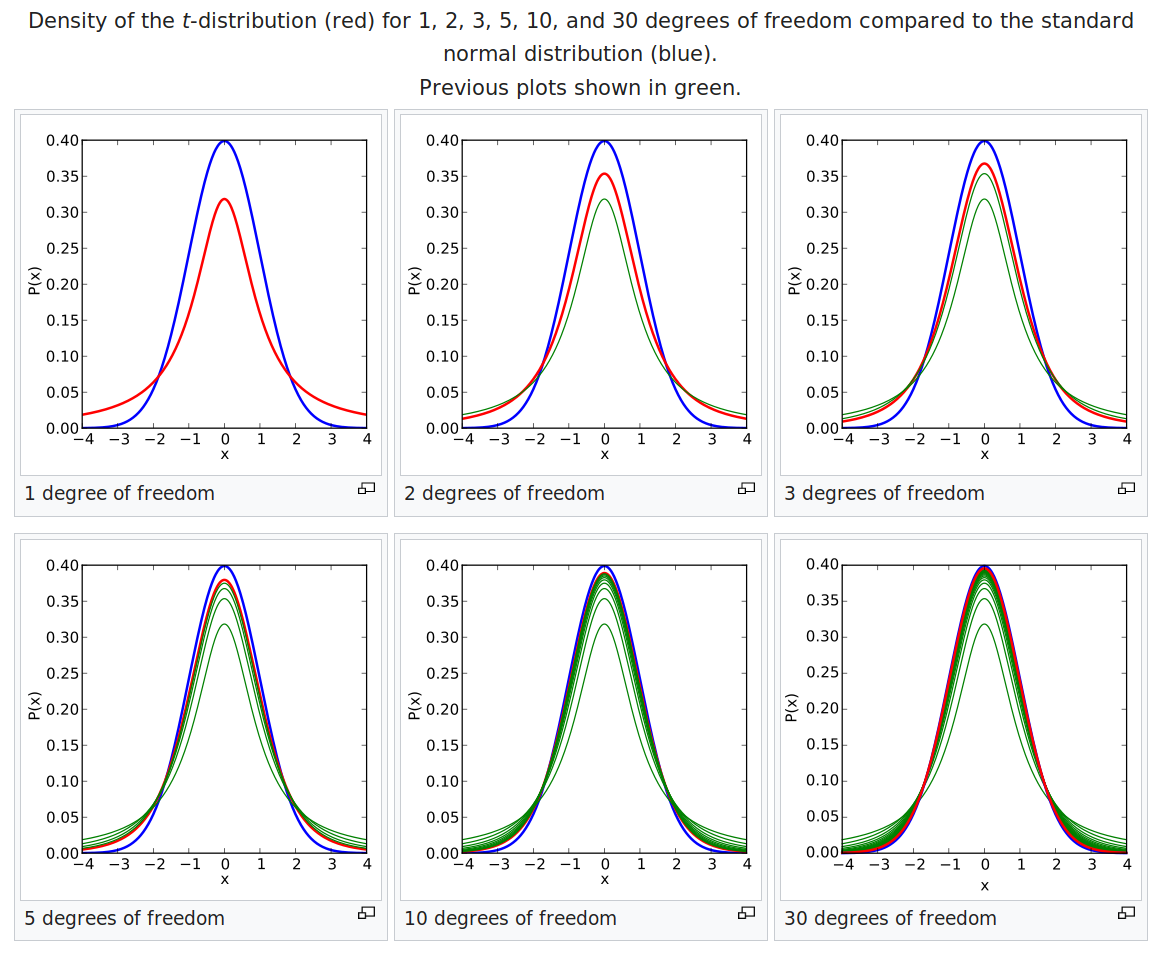
\includegraphics[width=0.7\textwidth]{t_distributions_wikipedia.png}\\ [-1.5ex]
      {\fontsize{10}{0}\selectfont \textbf{Source: Wikipedia}}

    \item t-statistic critical value table for lookup can be found \underline{\href{https://www.ruf.rice.edu/~bioslabs/tools/stats/ttable.html}{here}}.
      
    \end{itemize}
  \end{itemize}
  \newpage
% ----------------------------------------------------------------
% ANOVA
% ----------------------------------------------------------------
\item \textbf{ANOVA}
  \begin{itemize}
  \item Tests the variance of \emph{three or more groups of observations} for whether there is a significant difference between their means (i.e. probably not due to normal variation in the samples)
  \item The name stands for \emph{completely randomized one-way analysis of variance}
  \item Can be applied to cases where the groups are independent and random, the distributions are normal and the populations have similar variances
  \item A hypothesis test, where the null hypothesis is that the means of the groups are equal
  \item Central to ANOVA is a number called the $F$ statistic, which is essentially the ratio between inter-group variation and intra-group variation
  \item The F-statistic is compared with the critical value from a table called the F-table (based on the F-statistic distribution) as a means of deciding whether the null hypothesis should be accepted. The critical value depends on the required confidence level, the number of groups and the number of observations.
    \newpage
  \item Calculation of the F-statistic:
    $$ MSB = \dfrac{\sum_{i=1}^k n_i(\mean{x_i} - \mean{\mean{x}})^2}{k-1}$$
    $$ MSW = \dfrac{\sum_{i=1}^k (n_i - 1)s_i^2}{N-k}$$
    $$ F = \dfrac{MSB}{MSW}$$
    where $k$ is the number of groups, $N$ is the overall number of observations, $n_i$ is the number of observations in group $i$ and $s_i$ is the standard deviation within group $i$, $\mean{x_i}$ is the mean within group $i$ and $\mean{\mean{x}}$ is the overall mean.
  \item The F-distribution depends on two \textbf{degrees of freedom} values, which also need to be used when looking up the F-table:
    $$ df_{between} = k - 1$$
    $$ df_{within} = N - k $$

    \item A file containing an F-table can be found \underline{\href{http://www.stat.purdue.edu/~jtroisi/STAT350Spring2015/tables/FTable.pdf}{here}}.
    
  \end{itemize}
  \newpage

% ----------------------------------------------------------------
% PAGE CHI-SQUARE
% ----------------------------------------------------------------
\item \textbf{Chi-square} 
  \begin{itemize}
  \item Tests the independence of categorical variables (on the nominal or ordinal scale)
  \item Chi-square can also be used to test goodnes of fit for a distribution (but we are not looking at that here)
  \item A hypothesis test where the hypothesis is that there is no relationship between the variables
  \item The value on which the hypothesis test is based is: \\
    $$ \chi^2 = \sum_{i=1}^k\dfrac{(O_i - E_i)^2}{E_i} $$
    where $k$ is the number of cells (categories) in the contingency table for the two variables, $O_i$ is the observed frequency in cell $i$ and $E_i$ is the expected frequency for cell $i$. The expected cell frequency is calculated as:
    $$ E_i = \dfrac{n_{Ri} \times n_{Ci}}{n} $$
    where $n_{Ri}$ is the sum of frequencies in the entire row to which cell $i$ belongs, $n_{Ci}$ is the sum of frequencies in the column to which cell $i$ belongs and $n$ is the sum of frequencies across the entire table.
  \item The calculated $\chi^2$ value is compared with the critical value for the required confidence level and number of degrees of freedom ($df=(r-1)\times(c-1)$, where $r$ and $c$ are the number of rows and columns, respectively, in the contingency table) from the standard chi-square table. If the calculated $\chi^2$ is greater than the critical value, the null hypothesis is rejected and it is taken that \emph{there is a relationship} between the categorical variables.
    \item A Chi-square table can be found \underline{\href{http://303bha.duckdns.org/tudt/da/res/files/Labs/2\%20Relationships/images/2_1_1_chi_square_distribution_table.png}{here}}. 
  \end{itemize}
  \newpage
\end{itemize}


\newpage
\headersec{References}
Some pictures in this presentation were taken from the following books. The source for each picture is cited beside it. \\

\textbf{[MSD]} \emph{Making Sense of Data I: A Practical Guide to Exploratory Data Analysis and Data Mining}, by Glenn J. Myatt and Wayne P. Johnson, John Wiley \& Sons, 2014. \\



\end{document}
